%%\documentclass[handout]{beamer}
%\documentclass[aspectratio=169,13pt]{beamer}

%\newcommand{\dee}{\partial}

\newcommand{\bmat}[1]{\begin{bmatrix} \B{#1}_{11} & \B{#1}_{12} \\ \B{#1}_{21} & \B{#1}_{22}\end{bmatrix}}
\newcommand{\blmat}[1]{\begin{bmatrix} \B{#1}_{11} &  \\ \B{#1}_{21} & \B{#1}_{22}\end{bmatrix}}
\newcommand{\brmat}[1]{\begin{bmatrix} \B{#1}_{11} & \B{#1}_{12} \\ & \B{#1}_{22}\end{bmatrix}}
\newcommand{\bomat}[1]{\begin{bmatrix} {#1}_{11} & \B{#1}_{12} \\ \B{#1}_{21} & \B{\uppercase{#1}}_{22}\end{bmatrix}}
\newcommand{\blomat}[1]{\begin{bmatrix} {#1}_{11} & \\ \B{#1}_{21} & \B{\uppercase{#1}}_{22}\end{bmatrix}}
\newcommand{\bromat}[1]{\begin{bmatrix} {#1}_{11} & \B{#1}_{12} \\  & \B{\uppercase{#1}}_{22}\end{bmatrix}}

\DeclareMathOperator{\vcop}{vec}
\newcommand{\vc}[1]{\vcop\left(#1\right)}
\newcommand{\prm}{\mu}

\newcommand{\fl}{fl}
\newcommand{\asmcond}[1]{\smallskip{\it #1}\smallskip}
\newcommand{\amdcond}[1]{\smallskip{\it #1}\smallskip}
\newcommand{\algcond}[1]{\smallskip{\it #1}\smallskip}
\newcommand{\atsmcond}[1]{{\it #1}}
\newcommand{\atmdcond}[1]{{\it #1}}
\newcommand{\atlgcond}[1]{{\it #1}}
\newcommand{\afillnum}[1]{{\underline{ \ #1\ \ }}}

\mode<presentation>
{
  \usetheme{Malmoe}
}

\usepackage[english]{babel}
%
%\usepackage[latin1]{inputenc}
%
%\usepackage{times}
%\usepackage[T1]{fontenc}
% Or whatever. Note that the encoding and the font should match. If T1
% does not look nice, try deleting the line with the fontenc.

\usepackage{inconsolata}
\usepackage{listings}
\usepackage{bm}
\usefonttheme[onlymath]{serif}
\renewcommand\familydefault{\sfdefault}
\usepackage[sfdefault]{ClearSans} %% option 'sfdefault' activates Clear Sans as the default text font
%\usefonttheme{professionalfonts}

\usepackage{latexsym}
\usepackage{amsmath}
\usepackage{amssymb}
\usepackage{amsfonts}
\usepackage{graphics}
\usepackage{multicol}

\definecolor{darkred}{rgb}{0.8,0.2,0.2}
\newcommand{\coloremph}[1]{\textcolor{darkred}{\emph{#1}}}        % colored italics
\newcommand{\reshape}[2]{o_{#1}(#2)}        % colored italics
\newcommand{\ket}[1]{\lvert #1 \rangle}
\newcommand{\bra}[1]{\langle #1 \vert}
\newcommand{\transp}[2]{{#2}^{\langle  {#1} \rangle }}        % colored italics

% Miscellaneous special math symbols

% Big-oh notation - either Latex's calligraphic O or uppercase math italic O
\newcommand{\BIGOH}{\mathcal{O}}                              % big oh
%\newcommand{\BIGOH}{O}                                       % big oh
\newcommand{\BIGTHETA}{\Theta}                                % big theta

\newcommand{\sfrac}[2]{{#1}/{#2}}

% Various versions of the fraction one-half
% solidus 1/2 for superscripts:
\newcommand{\SHALF}{1/2}                                      % one-half power
% small 1/2 set case in displayed equations:
\newcommand{\HALF}{\mbox{\small $\frac{1}{2}$}}               % small one-half
\newcommand{\THRD}{\mbox{\scriptsize $\frac{1}{3}$}}          % small one-third
\newcommand{\TWOTH}{\mbox{\scriptsize $\frac{2}{3}$}}         % small two-thirds

% Machine epsilon - note that placement of subscript may need adjustment.
%\newcommand{\emach}{\epsilon_{\textrm{\scriptsize mach}}} % machine prec.
\newcommand{\emach}{\epsilon}

\newcommand{\lsapprox}{\cong}                             % least squares approx

% Real numbers - Prefer \mathbb{R} but it requires amsfonts.
%                Latex's calligraphic R will do if amsfonts are unavailable.
%                DO NOT use \Re, which gives old German fraktur R.
\newcommand{\Real}{\mathbb{R}}                                 % real numbers
\newcommand{\Cplx}{\mathbb{C}}                                 % complex numbers
\newcommand{\Poly}{\mathbb{P}}                                 % polynomials
\newcommand{\Float}{\mathbb{F}}                                % fl pt system
% Bold math fonts for vectors and matrices
\renewcommand{\Vec}[1]{\ensuremath{\bm{#1}}}                   % vector
\newcommand{\Mat}[1]{\ensuremath{\bm{#1}}}                     % matrix
\newcommand{\Op}[1]{#1}                              % operator
\newcommand{\loc}[1]{x_{#1}}                              % operator

% Loglike functions set in regular type
\newcommand{\diag}{\mathrm{diag}}                             % diagonal matrix
\newcommand{\cond}{\mathrm{cond}}                             % condition number
\newcommand{\sign}{\mathrm{sign}}                             % sign function
\newcommand{\Span}{\text{span}}                             % span of matrix
%\newcommand{\trace}{\mathrm{trace}}                           % trace of matrix
\DeclareMathOperator*{\trace}{trace}
\newcommand{\tentrace}[3]{\trace_{#1,#2}(#3)}
\renewcommand{\Re}{\mathrm{Re}}                               % real part
\renewcommand{\Im}{\mathrm{Im}}                               % imaginary part

% Fractions appearing in matrices - allows setting them case or solidus
%\newcommand{\mf}[2]{{#1 \over #2}}        % matrix fraction - set case
\newcommand{\mf}[2]{#1/#2}               % matrix fraction - set solidus


% Keywords for algorithm statements

\newcommand{\FOR}{\textbf{for}\ }
\newcommand{\TO}{\textbf{to}\ }
\newcommand{\IF}{\textbf{if}\ }
\newcommand{\THEN}{\textbf{then}\ }
\newcommand{\ELSE}{\textbf{else}\ }
\newcommand{\WHILE}{\textbf{while}\ }
\newcommand{\DO}{\textbf{do}\ }
\newcommand{\BEGIN}{\textbf{begin}\ }
\newcommand{\END}{\textbf{end}\ }
\newcommand{\STOP}{\textbf{stop}\ }
\newcommand{\AND}{\textbf{and}\ }
\newcommand{\OR}{\textbf{or}\ }

\newcommand{\comm}{\mathrm{comm}}
\newcommand{\comp}{\mathrm{comp}}
\newcommand{\idle}{\mathrm{idle}}
\newcommand{\msg}{\mathrm{msg}}
\newcommand{\len}{\mathrm{s}}
\newcommand{\route}{\mathrm{route}}
\newcommand{\mitem}{\medskip\item}
\newcommand{\sitem}{\smallskip\item}
\DeclareMathOperator*{\argmin}{argmin}

%Gets rid of headline

\setbeamertemplate{footline}{}

\setbeamertemplate{headline}{}
\beamertemplatenavigationsymbolsempty



\definecolor{mygreen}{rgb}{0,0.2,0}
\definecolor{mygray}{rgb}{0.5,0.5,0.5}
\definecolor{mymauve}{rgb}{0.58,0,0.82}
\definecolor{mypurple}{rgb}{0.38,0,0.32}
\definecolor{myblue}{rgb}{0.2,0,0.5}
\definecolor{darkgreen}{rgb}{0.2,0.6,0.2}
\definecolor{Brown}{rgb}{0.39, 0.09, 0.0}
\definecolor{Violet}{rgb}{0.38, 0.0, 0.63}
\definecolor{myvlgray}{rgb}{0.9,0.9,1.0}
\definecolor{mylgray}{rgb}{0.85,0.85,0.9}
\definecolor{darkgreen}{rgb}{0,0.4,0}
\definecolor{brown}{rgb}{.6,.1,.1}

\newcommand{\bemph}[1]{{\color{blue} \emph{#1}}}

\usepackage{mathtools}
\newcommand{\defeq}{\coloneqq}

\newcommand{\inti}[2]{[{#1},{#2}]}
\newcommand{\BF}{\mathbf}
\newcommand{\CF}{\mathcal}
\newcommand{\B}[1]{\bm{#1}}
\newcommand{\E}[1]{\bm{#1}}
\newcommand{\dis}{\displaystyle}
\newcommand{\lt}{\left}
\newcommand{\rt}{\right}

\newcommand{\cs}{H}

\DeclareMathOperator*{\rank}{rank}
\DeclareMathOperator*{\vecn}{vec}
\DeclareMathOperator*{\vecs}{vech}

\usepackage{eso-pic}
\newcommand{\cornertext}[1]{
  \AddToShipoutPictureFG*{
    \AtPageUpperLeft{\put(0,-10){\makebox[\paperwidth][r]{#1}}}  
   }%
}
\newcommand{\cornertexttwo}[2]{
  \AddToShipoutPictureFG*{
    \AtPageUpperLeft{\put(0,-10){\makebox[\paperwidth][r]{#1}}}  
    \AtPageUpperLeft{\put(0,-20){\makebox[\paperwidth][r]{#2}}}  
   }%
}
\newcommand{\linkdemo}[2]{{\footnotesize\href{https://relate.cs.illinois.edu/course/cs450-f18/f/demos/upload/#1/#2.html}{\color{Violet}{\it\textbf{Demo:} #2}\ }}}
\newcommand{\linkinclass}[2]{{\footnotesize\href{https://relate.cs.illinois.edu/course/cs450-f18/flow/#1/start/}{\color{darkgreen}{\it\textbf{Activity:} #2}\ }}}
\newcommand{\urcornerlinkinclass}[2]{\cornertext{\linkinclass{#1}{#2}}}
\newcommand{\dblurcornerlinkinclass}[4]{\cornertexttwo{\linkinclass{#1}{#2}}{\linkinclass{#3}{#4}}}
\newcommand{\urcornerlinkdemo}[2]{\cornertext{\linkdemo{#1}{#2}}}
\newcommand{\dblurcornerlinkdemo}[4]{\cornertexttwo{\linkdemo{#1}{#2}}{\linkdemo{#3}{#4}}}
\newcommand{\urcornerlinkdemoinclass}[4]{\cornertexttwo{\linkdemo{#1}{#2}}{\linkinclass{#3}{#4}}}



% CS 554 specific:

\newcommand{\tsync}{\alpha}
\newcommand{\tword}{\beta}
\newcommand{\tflop}{\gamma}

\newcommand{\bw}{w}

\newcommand{\tpl}[2]{{\bm{#1}}}
\newcommand{\vtpl}[3]{{\bm{#1}}_#3}
\newcommand{\perm}[2]{\lt[#1\rt]_{#2}}
\newcommand{\costyle}{\ttfamily\bfseries}
\newcommand{\cotext}[1]{{\costyle{#1}}}
\newcommand{\kwstyle}{\costyle\textcolor{mypurple}}
\newcommand{\kwtext}[1]{{\kwstyle{#1}}}
\newcommand{\emstyle}{\costyle\textcolor{myblue}}
\newcommand{\emtext}[1]{{\emstyle{#1}}}
\newcommand{\const}{}
\newcommand{\work}{Q}
\newcommand{\depth}{D}
\newcommand{\flops}{F}
\newcommand{\words}{W}
\newcommand{\syncs}{S}
\newcommand{\mem}{M}
\newcommand{\eff}{E}
\newcommand{\isofun}[1]{\tilde{\work}(p)}
\newcommand{\isomem}[1]{\tilde{\mem}(p)}
\newcommand{\pstrong}{p_s}
\newcommand{\pweak}{p_w}
\newcommand{\ALL}{\star }
\newcommand{\rmn}[2]{\mathbb{R}^{#1\times #2}}
\newcommand{\rn}[1]{\mathbb{R}^{#1}}
\newcommand{\err}{\varepsilon}
\newcommand{\mat}[1]{\begin{bmatrix} #1 \end{bmatrix}}
\newcommand{\mc}[1]{\mathcal{#1}}
\newcommand{\h}[2]{\mc{H}_{#1}(#2)}
\newcommand{\T}{T}%{\mathsf{T}}
\newcommand{\dn}[2]{\mc{M}_{#1}^{\uparrow}(#2)}
%\usepackage[colorlinks=false,urlbordercolor={1.0 1.0 1.0}]{hyperref}
%
%\lstset{ %
%  postbreak=false,
%%  backgroundcolor=\color{white},   % choose the background color; you must add \usepackage{color} or \usepackage{xcolor}
%  basicstyle=\costyle,        % the size of the fonts that are used for the code
%%  breakatwhitespace=false,         % sets if automatic breaks should only happen at whitespace
%%  breaklines=false,                 % sets automatic line breaking
%  captionpos=n,                    % sets the caption-position to bottom
%  commentstyle=\color{mygreen},    % comment style
%  deletekeywords={...},            % if you want to delete keywords from the given language
%  escapeinside={\%*}{*)},          % if you want to add LaTeX within your code
%  extendedchars=true,              % lets you use non-ASCII characters; for 8-bits encodings only, does not work with UTF-8
%  frame=none,                    % adds a frame around the code
%  keepspaces=true,                 % keeps spaces in text, useful for keeping indentation of code (possibly needs columns=flexible)
%  keywordstyle=\color{mypurple},       % keyword style
%  language=C++,                 % the language of the code
%  otherkeywords={*,...},            % if you want to add more keywords to the set
%  numbers=none,                    % where to put the line-numbers; possible values are (none, left, right)
%  numbersep=5pt,                   % how far the line-numbers are from the code
%  numberstyle=\tiny\color{mygray}, % the style that is used for the line-numbers
%  rulecolor=\color{black},         % if not set, the frame-color may be changed on line-breaks within not-black text (e.g. comments (green here))
%  showspaces=false,                % show spaces everywhere adding particular underscores; it overrides 'showstringspaces'
%  showstringspaces=false,          % underline spaces within strings only
%  showtabs=false,                  % show tabs within strings adding particular underscores
%  stepnumber=2,                    % the step between two line-numbers. If it's 1, each line will be numbered
%  stringstyle=\color{mymauve},     % string literal style
%  tabsize=2,                     % sets default tabsize to 2 spaces
%  title=\lstname,                   % show the filename of files included with \lstinputlisting; also try caption instead of title
%  keywordstyle=\emstyle
%}

\lstset{ %
  postbreak=false,
%  backgroundcolor=\color{white},   % choose the background color; you must add \usepackage{color} or \usepackage{xcolor}
  basicstyle=\footnotesize\costyle,        % the size of the fonts that are used for the code
%  breakatwhitespace=false,         % sets if automatic breaks should only happen at whitespace
%  breaklines=false,                 % sets automatic line breaking
  captionpos=n,                    % sets the caption-position to bottom
  commentstyle=\color{mygreen},    % comment style
  deletekeywords={privatei,shared},            % if you want to delete keywords from the given language
  escapeinside={\%*}{*)},          % if you want to add LaTeX within your code
  extendedchars=true,              % lets you use non-ASCII characters; for 8-bits encodings only, does not work with UTF-8
  frame=none,                    % adds a frame around the code
  keepspaces=true,                 % keeps spaces in text, useful for keeping indentation of code (possibly needs columns=flexible)
  keywordstyle=\footnotesize\color{mypurple},       % keyword style
  language=C++,                 % the language of the code
  otherkeywords={*,pragma},            % if you want to add more keywords to the set
  numbers=none,                    % where to put the line-numbers; possible values are (none, left, right)
  numbersep=5pt,                   % how far the line-numbers are from the code
  numberstyle=\footnotesize\color{mygray}, % the style that is used for the line-numbers
  rulecolor=\color{black},         % if not set, the frame-color may be changed on line-breaks within not-black text (e.g. comments (green here))
  showspaces=false,                % show spaces everywhere adding particular underscores; it overrides 'showstringspaces'
  showstringspaces=false,          % underline spaces within strings only
  showtabs=false,                  % show tabs within strings adding particular underscores
  stepnumber=2,                    % the step between two line-numbers. If it's 1, each line will be numbered
  stringstyle=\footnotesize\color{mymauve},     % string literal style
  tabsize=2,                     % sets default tabsize to 2 spaces
  title=\lstname,                   % show the filename of files included with \lstinputlisting; also try caption instead of title
  emph={MPI_Send,MPI_Recv,MPI_Comm,MPI_Comm_rank,MPI_Send,MPI_Comm_split,MPI_Init,MPI_Finalize,MPI_Status,MPI_COMM_WORLD,MPI_Datatype,MPI_Comm_size,MPI_FLOAT,mpi.h,omp,parallel,shared,private,default,reduction},
  emphstyle=\footnotesize\emstyle
}

\title{CS 450: Numerical Anlaysis\footnote{{\it These slides have been drafted by Edgar Solomonik as lecture templates and supplementary material for the book ``Scientific Computing: An Introductory Survey'' by Michael T. Heath (\href{http://heath.cs.illinois.edu/scicomp/notes/index.html}{{\color{blue} slides}}).}}}
\author{}
\institute{University of Illinois at Urbana-Champaign}




\subtitle{Initial Value Problems for Ordinary Differential Equations}
\date{}
\begin{document}

\begin{frame}
  \titlepage
\end{frame}

\section{Introduction to ODEs}
\begin{frame}{Ordinary Differential Equations}

\begin{itemize}
\item An \coloremph{ordinary differential equation (ODE)} usually describes time-varying system by a function $\B y(t)$ that satisfies a set of equations in its derivatives.

\tlgcond{
The general \coloremph{implicit} form is
\[\B g(t,\B y, \B y', \B y'',\ldots, \B y^{(k)}) = \B 0,\]
but we restrict focus on the \coloremph{explicit form},
\(\B y^{(k)} = \B f(t,\B y, \B y', \B y'',\ldots, \B y^{(k-1)}).\)
%The \coloremph{order} of an ODE is the highest-order derivative appearing in $g$, above $k$.
}
\item An ODE of any \coloremph{order} $k$ can be transformed into a first-order ODE,

\tlgcond{
\[\B u' = \begin{bmatrix} \B u_1' \\ \vdots \\ \B u_{k-1}'\\ \B u_k' \end{bmatrix} = \begin{bmatrix} \B u_2 \\ \vdots \\ \B u_{k}\\ \B f(t,\B u_1,\ldots, \B u_k) \end{bmatrix} \quad \text{where} \quad \B u_i(t)=\B y^{(i-1)}(t). \]
Consequently, we restrict our focus to systems of first-order ODEs.
Of particular importance are \coloremph{linear ODEs}, which have the form $\B y' =\B A(t) \B y$, whose \coloremph{coefficients} are said to be \coloremph{constant} if $\B A(t)=\B A$ for all $t$.

}

\end{itemize}

\end{frame}

\begin{frame}{Example: Newton's Second Law}

\begin{itemize}
\item $F=ma$ corresponds to a second order ODE,
\tlgcond{
\begin{align*}
F &= my''(t), \\
y''(t) &= F/m.
\end{align*}

}
\item We can transform it into a first order ODE in two variables:

\tlgcond{
\[\B u = \begin{bmatrix} y(t) \\ y'(t) \end{bmatrix},\]
\[\begin{bmatrix} u_1' \\ u_2' \end{bmatrix} = \B u' = \B f(t,\B u) = \begin{bmatrix} u_2 \\ F/m\end{bmatrix}.\]
}


\end{itemize}

\end{frame}

\section{Existence and Uniqueness of Solutions}
\begin{frame}{Initial Value Problems}

\begin{itemize}
\item Generally, a first order ODE specifies only the derivative, so the solutions are non-unique. An \coloremph{initial condition} addresses this:

\tlgcond{
\[\B y(t_0)=\B y_0\]
This condition yields an initial value problem (IVP), which is the simplest example of a \coloremph{boundary condition}.
}
\item Given an initial condition, an ODE must satisfy an integral equation for any given point $t$:

\tlgcond{
\[\B y(t) =\B y_0 + \int_{t_0}^t \B f(s,\B y(s)) ds,\]
In the special case that $\B y'=\B f(t)$, the integral can be computed directly by numerical quadrature to solve the ODE.
}

\end{itemize}

\end{frame}

\begin{frame}{Existence and Uniqueness of Solutions}

\begin{itemize}
\item For an ODE to have a unique solution, it must be defined on a closed domain $D$ and be \coloremph{Lipschitz continuous}:

\tlgcond{
\[\forall \B y, \B{\hat{y}} \in D, \quad ||\B f(t,\B{\hat{y}})-\B f(t,\B{y})|| \leq L || \B{\hat{y}} - \B{y}||,\]
i.e. the rate of change of the ODE should itself change continuously.
Any differentiable function $\B f$ is Lipschitz continuous with
 \[L=\max_{(t,\B y)\in D} ||\B J_{\B f}(t,\B y)||,\]
where $\B J_{\B f}$ is Jacobian of $\B f$ with respect to $\B y$.
}
\item The solutions of an ODE can be stable, unstable, or asymptotically stable:

\lgcond{
Perturbation to the input causes a perturbation to the solution that 
\begin{itemize}
\item has bounded growth for a stable ODE, 
\item unbounded growth for an unstable ODE, and
\item shrinks for an asymptotically stable ODE.
\end{itemize}
}

\end{itemize}

\end{frame}

\section{Stability and Error in ODEs}
\begin{frame}{Stability of 1D ODEs}

\begin{itemize}
\item The solution to the scalar ODE $y'=\lambda y$ is $y(t)=y_0e^{\lambda t}$, with stability dependent on $\lambda$:

\tlgcond{
\[\lim_{t\to\infty} y(t) = \begin{cases} \infty &: \lambda> 0 \text{\ (unstable)\ } \\ y_0 &: \lambda=0 \text{\ (stable)\ } \\ 0 &: \lambda<0 \text{\ (asymptotically stable)\ }\end{cases}\]
}
\item A constant-coefficient linear ODE has the form $\B y' = \B  A \B y$, with stability dependent on the real parts of the eigenvalues of $\B A$:

\lgcond{
\begin{itemize}
\item At a point $(t,\B y)$, any ODE can be approximated by a linear ODE of the form $\B z'= \B J_{\B f}(t,\B y)\B z$.
\mitem For general ODEs, stability can be ascertained locally by considering the eigenvalues of $\B J_{\B f}(t,\B y)$.
\end{itemize}
}

\end{itemize}

\end{frame}





%\begin{frame}{Initial Value Problems for ODEs}
%
%\begin{itemize}
%\item We restrict attention to first-order systems of ODEs and pay special attention to linear and constant-coefficient systems:
%
%\lgcond{
%An IVP for an ODE usually has the form $\B y'= \B f( t, \B y)$ with initial value $(t_0,\B y(t_0))$.
%A linear ODE $\B f$ has the form $\B f(t,\B y) = \B A(t) \B y(t)$, and is said to have constant coefficients if $\B A(t)$ does not vary with $t$.
%}
%
%\item Existence and uniqueness of a solution to an IVP is guaranteed over any domain $D$ on which $\B f$ is Lipschitz continuous:
%
%\lgcond{
%\[\exists L\in \mathbb{R}, ||\B f(t, \B y) - \B f(t,\B{\hat{y}})|| \leq L||\B y - \B{\hat{y}}||, \forall \B y, \B{\hat{y}}\in D\]
%which is stronger than continuity of $\B f$ (differentiability of $\B y$), but weaker than differentiability of $\B f$, i.e. $\B f$ can suddenly begin to change at a different rate.
%The constant $L$ bounds the rate at which similar solutions $\B y$ and $\B{\hat{y}}$ can diverge or converge.
%}
%
%\end{itemize}
%
%\end{frame}





\subsection{Explicit Methods}

\begin{frame}{Numerical Solutions to ODEs}
\urcornerlinkdemo{09-initial-value-problems}{Forward Euler stability}

\begin{itemize}
\item Methods for numerical ODEs seek to approximate $\B y(t)$ at $\{t_k\}_{k=1}^m$.

\lgcond{
Compute $\B{y}_k$ for $k\in\{1,\ldots,m\}$ so as to approximate $\B y(t_k)\approx \B{y}_k$.
For an IVP, typically form $\B{y}_{k+1}$ using $\B{y}_{k}$ or additionally (for multistep methods) $\B{y}_{k-1},\ldots$
}

\item Euler's method provides the simplest method (attempt) for obtaining a numerical solution:

\lgcond{
Approximation solution to ODE at $t_k+h$ by linear segment from $(t_k, \B y_k)$ with slope $\B f(t_k, \B y_k)$,
\[\B y_{k+1} = \B y_k +h_k\B f(t_k, \B y_k).\]
This approximation is the first order form of various models (Taylor series, finite differences, interpolation, quadrature, undetermined coefficients).
}

\end{itemize}

\end{frame}

\begin{frame}{Error in Numerical Methods for ODEs}

\begin{itemize}
\item Truncation error is typically the main quantity  of interest, which can be defined \coloremph{globally} or \coloremph{locally}:

\tlgcond{
\begin{itemize}
\item 
Global error is measured at all points
\[\B e_k = \B{y}_k - \B y(t_k).\]
\item Local error measures the deviation from the exact solution $\B u_{k-1}(t)$ passing through the previous point $(t_{k-1},\B{y}_{k-1})$,
\[\B l_k = \B{y}_k - \B u_{k-1}(t_k).\]
\end{itemize}
}
\item The \coloremph{order of accuracy} of a given method is one less than than the order of the leading order term in the local error $\B l_k$:

\lgcond{
\begin{itemize}
\item
Accuracy is of order $p$ if $\B l_k=O(h^{p+1}_k)$, for forward Euler $p=1$ since
\[\B y(t_{k+1}) = \B y(t_k) +h_k\B f(t_k, \B y(t_k)) + O(h_k^2),\]
so $\B l_k = O(h_k^2)$.
%\mitem 
%Euler's method is first order accurate by Taylor expansion analysis.
\end{itemize}
}

\end{itemize}

\end{frame}

%\begin{frame}{Convergence and Stability}
%
%
%\begin{itemize}
%\item Generally, we seek to approximate $\B y(t_k)$ for a set of points $t_k=t_0+kh$ by $\B y_k$:
%
%\lgcond{
%Would like to converge with decreasing step-size, i.e. $\lim_{h\to 0} \B{y}_k = \B y(t_k)$.
%Can measure global error (deviation from true solution) or local error (deviation of $\B{y}_k$ from $\B u_{k-1}(t_k)$ where $\B u_{k-1}(t_{k-1})=\B{y}_{k-1}$ and $\B u_{k-1}' = \B y'$).
%}
%
%\item Stability ascertains behavior as $t\to \infty$ either of the ODE itself or of a numerical method:
%
%\lgcond{
%\begin{itemize}
%\item For an ODE, stability identifies convergence/divergence of perturbed solutions.
%\sitem For a numerical method, it identifies step-size bounds necessary to ensure the method converges along with the ODE.
%\sitem If a method is stable, the local error is a trustworthy metric of global error.
%\sitem A \coloremph{stiff} ODE is a convergent ODE with rapidly varying small components, which poses a challenge for stability of methods.
%\end{itemize}
%}
%
%
%\end{itemize}
%
%\end{frame}

\begin{frame}{Accuracy and Taylor Series Methods}

\begin{itemize}
\item By taking a degree-$r$ Taylor expansion of the ODE in $t$, at each consecutive $(t_k,\B{y}_k)$, we achieve $r$th order accuracy.

\lgcond{
We can bound the local approximation error as the error in the Taylor expansion, 
\[\B y(t_k+h) = \B y(t_k) + \B y'(t_k)h + \cdots + \B y^{(r)}(t_k)h^{r-1}/r!\]
which is $O(h^{r+1})$,  leading to $O(h^r)$ accuracy in the approximation to $\B f(t,\B y)$.
Euler's method is a first-order Taylor series method.
}

\item Taylor series methods require high-order derivatives at each step:

\lgcond{
\begin{itemize}
\item Analytic differentiation is expensive, so seek to approximate.
\mitem Can perform a finite-differencing approximation by evaluating at points near $(t_k,\B{y}_k)$ (multi-stage methods) or simply using previous points, e.g. $(t_{k-1},\B{y}_{k-1})$ (multi-step methods).
\end{itemize}
}


\end{itemize}

\end{frame}




\subsection{Stability Regions}
\begin{frame}{Growth Factors and Stability Regions}

\dblurcornerlinkdemo{09-initial-value-problems}{Stability regions}{09-initial-value-problems}{Stiffness}
\begin{itemize}
\item Stability of an ODE method discerns whether local errors are amplified, deamplified, or stay constant:

\lgcond{
%A method for an ODE with stable solutions can be unstable.
\begin{itemize}
\item A method is stable if the \coloremph{growth factor} of the error is less than or equal to one.
\mitem The \coloremph{stability region} for a method describes the step-size conditions necessary for stability in terms of 
  \begin{itemize}
  \item
  the step size $h$ (assuming its constant) and 
  \item 
  eigenvalues $\lambda$, usually as a function of $h\lambda$.
  \end{itemize}
\end{itemize}
}

\item Basic stability properties follow from analysis of linear scalar ODE, which serves as a local approximation to more complex ODEs.

\lgcond{
\begin{itemize}
\item
Consider forward Euler for the ODE $y'=\lambda y$, where
\[y_{k+1} = y_k + h \lambda y_k = \underbrace{(1+h\lambda)}_\text{growth factor}y_k.\]
\item 
Euler's method requires $|1+h\lambda| \leq 1$ to be stable, which implies $-2\leq h\lambda \leq 0$
\mitem
The global error then satisfies
\[ e_k =  l_k + (1+h\lambda) e_{k-1}.\]
% for real $\lambda$.
\end{itemize}
}

\end{itemize}

\end{frame}

\begin{frame}{Stability Region for Forward Euler}

\begin{itemize}
\item
The stability region of a general ODE constrains the eigenvalues of $h\B J_{\B f}$
\lgcond{
\begin{itemize}
\item The Mean Value Theorem implies that
\[ \exists \B{\xi}, \ \text{such that} \  \B f(t_k,\B y_k) - \B f(t_k, \B y(t_k)) = \B J_{\B f}(t_k, \B{\xi})(\B y_k - \B y(t_k))\]
and we know $||\B J_{\B f}(t_k, \B{\xi})||_2$ is bounded by Lipschitz continuity.
\mitem Consequently the growth factor for Forward Euler is 
\(\B I + h_k\B J_{\B f}(t_k, \B{\xi}).\)
\mitem The global error then satisfies
\[\B e_k = (\B I + h_k\B J_{\B f}(t_k, \B{\xi}))\B e_{k-1} + \B l_k.\]
\item Forward Euler is asymptotically stable if the spectral radius of the growth factor is less than one, which implies that the eigenvalues of $h_k\B J_{\B f}(t_k, \B{\xi})$ must always lie within a stability region that is a circle on the complex plane centered at $-1$ with radius $1$.
{

\centering

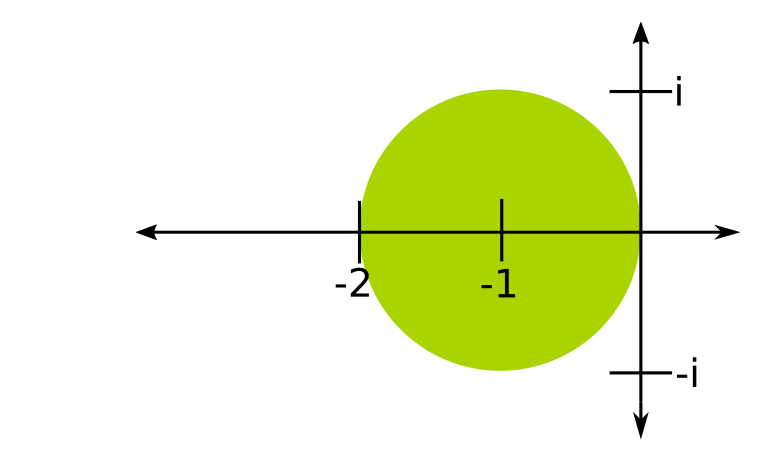
\includegraphics[width=1.5in]{diagrams/forward_euler_stability_region}

}
\end{itemize}
}
\lgcond{}
\end{itemize}

\end{frame}


\section{Implicit Schemes}
\begin{frame}{Backward Euler Method}
\urcornerlinkdemoinclass{09-initial-value-problems}{Backward Euler stability}{inclass-backward-euler}{Backward Euler Method}

\begin{itemize}
\item Implicit methods for ODEs form a sequence of solutions that satisfy conditions on a local approximation to the solution:

\tlgcond{
\smallskip
The most basic implicit method is the \coloremph{backward Euler} method
\[\B y_{k+1} = \B y_k + \B h_k\B f(t_{k+1},\B y_{k+1}),\]
which solves for $\B y_{k+1}$ so that a linear approximation of the solution at $t_{k+1}$ passes through the point $(t_k,\B y_k)$.
Just like forward Euler, first-order accuracy is achieved by the linear approximation.
}

\item The stability region of the backward Euler method is the left half of the complex plane:

\lgcond{
Such a method is called \coloremph{unconditionally stable}.
Note that the growth factor can be derived via
\[y_{k+1} = y_k + h\lambda y_{k+1}= \frac{1}{1-h\lambda}y_k,\]
and satisfies $|1/(1-h\lambda)|\leq 1$ so long as $h\lambda\leq 0$.
}

\end{itemize}

\end{frame}

\begin{frame}{Trapezoid Method}

\begin{itemize}
\item A second-order accurate implicit method is the \coloremph{trapezoid method}

\lgcond{
\[\B y_{k+1} = \B y_k + \B h_k(\B f(t_{k},\B y_{k}) + \B f(t_{k+1},\B y_{k+1}))/2,\]
\begin{itemize}
\item This method takes the average of the backward and forward Euler steps.
\mitem Its growth factor is $\frac{1+h\lambda/2}{1-h\lambda/2}.$
\mitem Since $\left|\frac{1+h\lambda/2}{1-h\lambda/2}\right| \leq 1$ for any $\lambda <0$, the method is unconditionally stable.
\end{itemize}
}

\item Generally, methods can be derived from quadrature rules: 

\lgcond{
\begin{itemize}
\item Evaluate or approximate $\B f$ at a set of points near $(t_k,\B y_k)$.
\mitem Use weights from a given quadrature rule to approximate solution to local integral equation.
\mitem Finding appropriate quadrature nodes is hard, implicit methods in effect solve for them.
\end{itemize}
}

\end{itemize}

\end{frame}

\section{High-Order Methods}
\subsection{Runge-Kutta Methods}
\begin{frame}{Multi-Stage Methods}

\begin{itemize}
\item \coloremph{Multi-stage methods} construct $\B{y}_{k+1}$ by approximating $\B y$ between $t_k$ and $t_{k+1}$:

\lgcond{
\begin{itemize}
\item \coloremph{Runge-Kutta methods} are the most well-known family of these, simple example is \coloremph{Heun's method},
\begin{align*}
\B{y}_{k+1} = \B{y}_k + h\bigg[\underbrace{\B f(t_k,\B y_k)}_{\B v_1}/2 + \B f\Big(t_k+h,\B y_k +h \underbrace{\B f(t_k,\B y_k)}_{\B v_1} \Big)/2\bigg].
\end{align*}
\item We can think of the above method as employing the trapezoid quadrature rule.
\mitem The difference between Heun's method and the (implicit) trapezoid method is that we evaluate at $\B f(t_k+h,\B y_k +h\B v_1)$ rather than working with the implicit value of $\B f(t_k+h,\B y_{k+1})$.
\end{itemize}
}
\item The 4th order Runge-Kutta scheme is particularly popular:

\algcond{
This scheme uses Simpson's rule,
\begin{alignat*}{2}
\B{y}_{k+1} &= \B{y}_k + (h/6)(\B v_1 + 2\B v_2 + 2\B v_3 +\B v_4) \\
\B v_1 &= \B f(t_k, \B y_k), \quad \quad
&&\B v_2 = \B f(t_k +h/2, \B y_k + (h/2)\B v_1), \\
\B v_3 &= \B f(t_k +h/2, \B y_k + (h/2)\B v_2), \quad \quad 
&&\B v_4 = \B f(t_k + h, \B y_k + h\B v_3).
\end{alignat*}
}
\end{itemize}
\end{frame}



\begin{frame}{Runge-Kutta Methods}
\urcornerlinkdemo{09-initial-value-problems}{Dissipation in Runge-Kutta Methods}

\begin{itemize}
\item %To compute $\B{y}_{k+1}$ 
Runge-Kutta methods evaluate $\B f$ at $t_k+c_ih$ for $c_0,\ldots, c_r\in[0,1]$, %$\B y_{ki})\}_{i=0}^{r}$ where $t_{ki}\in[t_k,t_{k+1}]$

%A Runge-Kutta method can be derived as a quadrature rule
\begin{align*}
\B{u}_{k}(t_{k+1}) &= \B{y}_{k} + \int_{t_k}^{t_{k}+h} \B f(s,\B y(s)) ds 
\quad\approx\quad \B{y}_{k} + h\sum_{i=0}^{r-1} w_i \B f(t_{k}+c_ih, \B{\hat{y}}_{ki}),
\end{align*}
\tlgcond{
where $\{(c_i,w_i)\}_{i=0}^r$ are quadrature (node, weight) pairs.
%, but we still have flexibility in choosing $\B{y}_{ki}$.
}
\item A general family of Runge Kutta methods can be defined by
\[\B{\hat{y}}_{ki} =\B{y}_{k} +h\sum_{j}a_{ij}\B f(t_{k}+c_ih, \B{\hat{y}}_{kj}).\]
\tlgcond{
Runge Kutta methods can then be represented by a \coloremph{Butcher tableau},
\[
\renewcommand\arraystretch{1.2}
\begin{array}
{c|cccc}
\B c & \B A \\
\hline
& \B w^T
\end{array} 
\quad \text{e.g. for RK4 $\B A$ has a single subdiagonal,} \quad
{\tiny
\begin{array}
{c|cccc}
0\\
\sfrac{1}{2} & \sfrac{1}{2}\\
\sfrac{1}{2} &0 &\sfrac{1}{2} \\
1& 0& 0& 1\\
\hline
& \sfrac{1}{6} &\sfrac{1}{3} &\sfrac{1}{3} &\sfrac{1}{6} 
\end{array}
}
\]
If $\B A$ is strictly lower triangular ($a_{ij}=0$ for $j\geq i$), the scheme is explicit, if $\B A$ is lower-triangular then it is diagonally implicit, and otherwise implicit.
}
\lgcond{}
\end{itemize}
\end{frame}


\begin{frame}{Properties of Runge-Kutta and Extrapolation Methods}

\begin{itemize}
\item Runge-Kutta methods are \coloremph{self-starting}, but are harder to use to obtain error estimates.

\algcond{
\begin{itemize}
\item Self-starting means that we only need $\B{y}_{k}$ to form $\B{y}_{k+1}$.
\mitem Embedded Runge-Kutta schemes provides 4th + 5th order results, yielding an error estimate.
\end{itemize}
}

\item \coloremph{Extrapolation methods} achieve high accuracy by successively reducing step-size.

\algcond{
Use single-step method with step sizes $h,h/2,h/4,...$ to approximate solution at $t_k+h$.
}


\end{itemize}
\end{frame}

\subsection{Multistep Methods}
\begin{frame}{Multistep Methods}

\begin{itemize}
\item \coloremph{Multistep methods} employ $\{\B{y}_{k}\}_{i=0}^k$ to compute $\B{y}_{k+1}$:

\lgcond{
Linear multistep methods have the form,
\[\B{y}_{k+1} =\sum_{i=1}^m \alpha_i\B{y}_{k+1-i}+h\sum_{i=0}^m\beta_i\B f(t_{k+1-i},\B{y}_{k+1-i}).\]
Interpolation is used to determine each $\alpha_i$ and $\beta_i$, method is explicit if $\beta_0=0$.
}

\item Multistep methods are not self-starting, but have practical advantages:

\lgcond{
\begin{itemize}
\item
Can be initiated by Runge-Kutta methods.
\mitem 
They require few function evaluations.
\mitem 
Generalize to non-uniformly-spaced points (\coloremph{multivalue methods}).
\end{itemize}
}


\end{itemize}
\end{frame}





%\end{document}

%\end{document}\end{document}
